\documentclass{beamer}
%\usetheme{Madrid}
%\usetheme{Berlin}
%\usepackage{german}
%\usepackage[latin1]{inputenc}
%\usepackage[T1]{fontenc}
%\mode<presentation>
 %{
 \usetheme{Madrid}
 \setbeamercolor*{palette primary}{use=structure,fg=black,bg=p7408C}
 \setbeamercolor*{palette secondary}{use=structure,fg=black,bg=p7406U}
 \setbeamercolor*{palette tertiary}{use=structure,fg=black,bg=p716C}
 %}
 
 \definecolor{p7408C}{HTML}{F6BE00}
  \definecolor{p7406U}{HTML}{FCB315}
 \definecolor{pyelloy}{HTML}{F6C100}
 \definecolor{p716C}{HTML}{F17C0E}
 
  \definecolor{p8C}{HTML}{A19589}
 \setbeamercolor{itemize item}{fg=p8C} % all frames will have red bullets
 \setbeamertemplate{itemize item}[triangle]
 \setbeamertemplate{itemize subitem}{\color{p7408C}$\blacktriangleright$}

\setbeamercolor{block title}{bg=p7408C,fg=black}

\usepackage{etex}
\usepackage{tikz,pgfplots}
\usepackage{picture}

%\usepackage{german}
%\usepackage[latin1]{inputenc}
\usepackage[T1]{fontenc}
\usepackage{booktabs}
\usepackage{graphicx}
\usepackage{epsfig}
\usepackage{changebar}
\usepackage{amsmath}
\usepackage{mathtools}
\usepackage[T1]{fontenc}
\usepackage[ansinew]{inputenc}
\usepackage{setspace}
\usepackage{multicol}
\usepackage{multirow}
\usepackage{dcolumn}
\usepackage{color}
\usepackage{colortbl}
\definecolor{lightgray}{gray}{0.8}
\definecolor{lightblue}{rgb}{0.8,0.8,0.8}
\usepackage{hyperref}
\usepackage{xcolor} 
\usepackage{array} 
\usepackage{subfig}
\usepackage{makecell}
\usetikzlibrary{arrows,positioning} 


\graphicspath{{/Users/jupiter/Dropbox/elements/coala/graphs/}{../../../../Dropbox/elements/spatialrebels/graphs/}{../../../../Dropbox/elements/spatialrebels/graphspres/}}



\begin{document}

\title[UCL]
{
Interdependent conflict escalation and duration: Taking into account interdependencies between rebel organizations}
\author[Santa Fe Workshop]
{
Nils Metternich\\
\footnotesize{\emph{COnflict Analysis LAb (COALA)}}
} 
\institute[]
{		Department of Political Science\\
		University College London\\
		n.metternich@ucl.ac.uk\\[4ex]
		}

\date{\today}

\begin{frame}
\titlepage
\end{frame}


\begin{frame}{Overview}
\begin{itemize}
\item Main argument: Need to take into account interdependencies between countries and organizations to:
\begin{itemize}
\item explain spread of violence 
\item explain interdependent dynamics (e.g. free-riding, outbidding etc)
\item and make accurate predictions
\end{itemize}
\item Presentation includes work with 
\begin{itemize}
\item Julian Wucherpfennig (Hertie School of Governance)
\item Elio Amicarelli (UCL)
\item Altaf Ali (UCL)
\item Gokhan Ciflikli (LSE)
\item Martin Steinwand (Stony Brook (University of Essex))
\item Bahar Leventoglu (Duke University)
\item Michael D. Ward (Duke University)
\item Shahryar Minhas (Michigan State)
\item Cassy Dorff (University of New Mexico)
\end{itemize}
\end{itemize}
\end{frame}

\begin{frame}{Actors and their Interactions}{Theoretical advances and empirical limitations}
\begin{center}
Monadic analysis $\rightarrow$ Dyadic analysis $\rightarrow$ Network analysis\\
\includegraphics[scale=0.45,angle=90]{network_104b.pdf}\\
\tiny{
\begin{tabular}{lll}
Collier and Hoeffler (2000) & Cunningham et al. (2009) & Current \\
Fearon and Laitin (2003)   & Wucherpfennig et al. (2012)  \\
Bates et al. (2005)    & Bapat and Bond (2012)     \\
Cunningham (2006)& Walter (2009)\\
Gleditsch et al. (2002) & Bakke et al. (2012)\\
Hegre et al. (2001) & Steinwand (2011)\\
& Cunningham (2013)\\
\end{tabular}}
\end{center}
\end{frame}

%\begin{frame}{Predictive turn in conflict studies}
%\begin{minipage}{2.1in}
%\begin{tiny}
%\begin{itemize}
%\item Gurr and Lichbach, 1986
%\item O'brien, 2002
%\item Schrodt, 2006
%\item Goldstone et al., 2010
%\item Ward, 2010
%\item Weidmann and Ward, 2010
%\item Schneider, Gleditsch and Carey, 2011
%\end{itemize}
% \end{tiny}
%\end{minipage}
%\begin{minipage}{2.5in}
%\begin{tiny}
%\begin{itemize}
%\item De Mesquita, 2011
%\item Ward et al., 2013
%\item Gleditsch and Ward, 2013
%\item Hegre et al., 2013
%\item Bell et al., 2013
%\item Brandt, Freeman and Schrodt, 2014
%\item Muchlinski et al., 2016
%\end{itemize}
% \end{tiny}
%\end{minipage}
%
%\begin{block}{Characteristics of predictive approaches} 
%\begin{itemize}
%\item $Y=f(X)+\epsilon$
%\item Focus on $\hat{Y}$ rather than $\hat{\beta}$
%\item $\hat{Y}=\hat{f}$
%\end{itemize}
%\end{block}
%\end{frame}
%
%
%\begin{frame}{Role of forecasting}
%Scientifically:
%\begin{itemize}
%\item Theory testing
%\item Theory building
%\item Outcome prediction 
%\end{itemize}
%Policy oriented:
%\begin{itemize}
%\item Policy prescriptive 
%\item Early warning
%\end{itemize}
%\footnotesize{Note: Data development and theory}
%\end{frame}
%
%\begin{frame}{Approaches and tradeoffs}
%\begin{center}
%\begin{tikzpicture}
%  \draw[->] (0,0) -- (4,0);
%  \draw[<-]  (0,4) -- (0,0) ;
%\node at (2,0) [below=.2] {Flexibility};
%\node at (0,2) [rotate=90,above=.2] {Interpretability};
%\node at (1,3) [above=.2] {GLM};
%\node at (3,1) [above=.2] {RF};
%\end{tikzpicture}
%\end{center}
%\end{frame}



\begin{frame}{How to think about interdependencies}{Country or actor level}
\only<1>{From a network perspective:}
\centering
\only<2>{
\scalebox{1}{
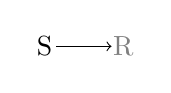
\begin{tikzpicture}
%Step 1
\draw [fill] (0,0)  node {S};
\draw [fill=gray,gray] (1,0) node {R};
\draw [->] (0.15,0) -- (0.85,0);
\end{tikzpicture}}}

\only<3>{
\scalebox{1}{
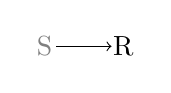
\begin{tikzpicture}
%Step 1
\draw [fill=gray,gray] (0,0)  node {S};
\draw [fill] (1,0) node {R};
\draw [->] (0.15,0) -- (0.85,0);
\end{tikzpicture}}}

\only<4>{
\scalebox{1}{
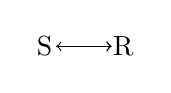
\begin{tikzpicture}
%Step 1
\draw [fill] (0,0)  node {S};
\draw [fill] (1,0) node {R};
\draw [->] (0.15,0) -- (0.85,0);

%Step2
\draw [<->] (0.15,0) -- (0.85,0);

\end{tikzpicture}}}


\only<5>{
\scalebox{1}{
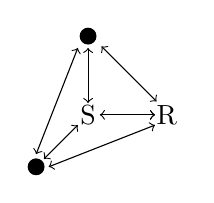
\begin{tikzpicture}
%Step 1
\draw [fill] (0,0)  node {S};
\draw [fill] (1,0) node {R};
\draw [->] (0.15,0) -- (0.85,0);

%Step2
\draw [<->] (0.15,0) -- (0.85,0);

%Step3

\draw [fill] (0,1) circle [radius=0.1];
\draw [fill] (-0.66,-0.66) circle [radius=0.1];

%\draw [fill=white,white] (2,0) circle [radius=0.1];
%\draw [fill=white,white] (-2,0) circle [radius=0.1];

\draw [<->] (0,0.15) -- (0,0.85);
\draw [<->] (-0.13,-0.13) -- (-0.56,-0.56);
\draw [<->] (-0.66,-0.5) -- (-.13,0.85);
\draw [<->] (-0.5,-0.66) -- (0.85,-.13);
\draw [<->] (0.17,.87) -- (.87,.17);
\end{tikzpicture}}}



\begin{itemize}
\item Sender
\item Receiver
\item Dyad
\item Second and third-order effects
%\only<5>{
%\begin{itemize}
%\item E.g. balancing. 
%\end{itemize}
%}
\end{itemize}

\end{frame}



\begin{frame}
\centering
\begin{table}
\caption{Analyzing interdependencies and the link between theory (utility of units) and empirical model. Arrows describe strategic interdependencies between actors.}
\label{tab:4by4}
\scalebox{0.72}{%
\begin{tabular}{l|c|l|l}
Type &Representation& Rebels' Utility& $y= \hdots +\epsilon$\\
\hline
Aggregate &
\begin{tikzpicture}
\draw [fill=gray,gray] (0,0) circle [radius=0.1];
\draw [fill=white,white] (2,0) circle [radius=0.1];
\draw [fill=white,white] (-2,0) circle [radius=0.1];
\draw [fill=white,white] (0,0.75) circle [radius=0.1];
\draw [fill=white,white] (0,-0.75) circle [radius=0.1];
\end{tikzpicture}
& $U_{i}(X)$ & $X\beta$ \\
\hline 
Dyadic & 
\begin{tikzpicture}
\draw [fill=gray,gray] (0,0) circle [radius=0.1];
\draw [fill] (1,0) circle [radius=0.1];
\draw [fill=white,white] (2,0) circle [radius=0.1];
\draw [fill=white,white] (-2,0) circle [radius=0.1];
\draw [<->] (0.15,0) -- (0.85,0);
\draw [fill=white,white] (0,0.75) circle [radius=0.1];
\draw [fill=white,white] (0,-0.75) circle [radius=0.1];
\end{tikzpicture}
& $U_{i}(X,Z)$ & $X\beta$+$Z\zeta$ \\
\hline 
K-dyads & 
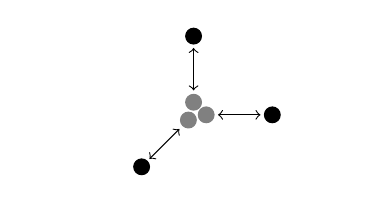
\begin{tikzpicture}
\draw [fill=gray,gray] (0,.16) circle [radius=0.1];
\draw [fill=gray,gray] (.16,0) circle [radius=0.1];
\draw [fill=gray,gray] (-.066,-.066) circle [radius=0.1];
\draw [fill] (0,1) circle [radius=0.1];
\draw [fill] (-0.66,-0.66) circle [radius=0.1];
\draw [fill] (1,0) circle [radius=0.1];
\draw [fill=white,white] (2,0) circle [radius=0.1];
\draw [fill=white,white] (-2,0) circle [radius=0.1];
\draw [<->] (0.31,0) -- (0.85,0);
\draw [<->] (0,0.31) -- (0,0.85);
\draw [<->] (-0.18,-0.18) -- (-0.56,-0.56);
\end{tikzpicture}

& $U_{i}(X,Z,K)$ & $X\beta$+$Z\zeta$+$K\kappa$ \\
\hline 
K-adic & 
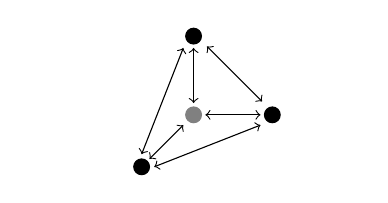
\begin{tikzpicture}
\draw [fill=gray,gray] (0,0) circle [radius=0.1];
\draw [fill] (0,1) circle [radius=0.1];
\draw [fill] (-0.66,-0.66) circle [radius=0.1];
\draw [fill] (1,0) circle [radius=0.1];
\draw [fill=white,white] (2,0) circle [radius=0.1];
\draw [fill=white,white] (-2,0) circle [radius=0.1];
\draw [<->] (0.15,0) -- (0.85,0);
\draw [<->] (0,0.15) -- (0,0.85);
\draw [<->] (-0.13,-0.13) -- (-0.56,-0.56);
\draw [<->] (-0.66,-0.5) -- (-.13,0.85);
\draw [<->] (-0.5,-0.66) -- (0.85,-.13);
\draw [<->] (0.17,.87) -- (.87,.17);
\end{tikzpicture}
& $U_{i}(X,Z,Y_{j},W)$ & $X\beta$+$Z\zeta$+$K\kappa$+$\rho Wy$ \\
\end{tabular}}
\end{table}
\end{frame}


\begin{frame}{Rebels and terrorist organizations are not alone}
\begin{itemize}
\item Interdependencies in conflicts
\begin{itemize}
\item Interdependent escalation
\item Interdependent duration
\end{itemize}
\end{itemize}
\end{frame}




\begin{frame}{Multiple Actors and Civil War}{Syrian Free Army}
Coalition of:
\begin{itemize}
\item Syria Revolutionaries Front
\item Hazzm Movement
\item Southern Command 
\item First Army
\item Yarmouk Brigade
\item Dawn of Freedom Brigades
\end{itemize}
\end{frame}


%\begin{frame}{Multiple Actors and Civil War}{Additional recent examples}
%Coalition of:
%\begin{itemize}
%\item Yemen
%\item Iraq
%\item Afghanistan 
%\item Libya
%\item Etc.
%\end{itemize}
%\end{frame}



\begin{frame}{Multiple Actors and Civil War}
\framesubtitle{Some stylized facts}

\begin{itemize}
    \item Civil conflicts typically involve several rebel groups and last longer\\ (e.g. Cunningham, 2006).
    \item Rebel groups form coalitions to fight the government\\ (e.g. Christia, 2012).
    \item Coalitions splinter, leading to continued fighting\\ (e.g. Bakke et al, 2012).
\end{itemize}

\vspace{.6cm}
{\bf Problems}
\begin{itemize}
    \item Policy related: Conflicts with more actors are harder to resolve (Cunningham 2006).
    \item Research literature: Existing theoretical \& empirical models of civil war typically only look at \alert{dyadic interactions}.
\end{itemize}
$\Rightarrow$ Need to account for strategic interactions to explain rebel fighting durations

\end{frame}


\begin{frame}
\begin{figure}[ht!]
\centering
\includegraphics[scale=0.45]{overlap_cases.pdf}
\caption{Rebel organization activity during selected UCDP armed conflicts.
%: Examples Chad $(UCDP ID=91)$, Congo $(UCDP ID=214)$, Uganda $(UCDP ID=118)$, and Guatemala $(UCDP ID=36)$. 
Each row represents a separate rebel organization as defined by a unique UCDP  $SideB$ for each rebel organization.}
\label{fig:example}
\end{figure}
\end{frame}

\begin{frame}{Interdependent escalation}
\centering
\includegraphics[scale=.4]{../../../../Dropbox/elements/coala/graphs/ANG.pdf}
\end{frame}

\begin{frame}{Interdependent escalation}
\centering
\includegraphics[scale=.4]{../../../../Dropbox/elements/coala/graphs/AFG.pdf}
\end{frame}

\begin{frame}{Interdependent escalation}
\centering
\includegraphics[scale=.4]{../../../../Dropbox/elements/coala/graphs/IRQ.pdf}
\end{frame}





\begin{frame}{Yet to Date...}
Strategic interaction is not systematically integrated in formal and empirical models, despite widespread agreement that it matters (e.g. Walter 2009, Cunningham 2006).
\end{frame}

\begin{frame}{Our Contribution (Metternich and Wucherpfennig, under review)}
First study that provides \textit{both} a
\begin{itemize}
\item theoretical model and
\item an empirical model
\end{itemize}
of strategic rebel group interdependence.\\ 

\begin{enumerate}
\item Showing that civil wars are generally dominated by competition dynamics.
\item However, conflict of public good provision (e.g. separatist conflicts) we see less competition
\end{enumerate}
\end{frame}



\begin{frame}{Public Goods $\rightarrow$ Problems}
\begin{itemize}
\item Fighting efforts against the government by one group that weaken the government will increase the chances of all other to obtain a favorable outcome
\item Rebel organizations formalize cooperation through alliances to avoid mutual exploitation (e.g., Bapat \& Bond 2012)
\item[]
\item[$\rightarrow$] Rebel organizations face incentives to underprovide (free-ride).
\item[$\rightarrow$] Fighting is a strategic substitute.
\end{itemize}
\end{frame}


\begin{frame}{Why Compete?}
\begin{itemize}
\item Cunningham, Bakke \& Seymour 2012, Fjelde \& Nillson 2012: political relevance, competition for resources (process-oriented)
\item Outcome-focused: $\rightarrow$ division of the spoils
\item Taking control of the post-conflict government: private or club good
\item Who gets what? 
\begin{enumerate}
\item Contest over relative survival: ``last rebel standing''
\begin{itemize}
\item Outlast competitors
\item Signal strength (attrition)
\end{itemize}
\item Division of spoils related to relative contribution
\begin{itemize}
\item Burden bearing compensated through spoils share
\end{itemize}
\end{enumerate}
\item Competition through fighting the government
\item[]
\item[$\rightarrow$] Rebel organizations have incentives to over-provide
\end{itemize}
\end{frame} 




\begin{frame}
\frametitle{Spatial Econometrics for Durations}

AFT Duration Model
\begin{equation}
y=\mathbf{X\beta} +\frac{1}{\lambda}u 
\end{equation}
where:
\begin{itemize}
\item $y=$ logged time until failure
\item $X=$ covariates
\item $u=$ stochastic error (i.i.d), scaled by a shape parameter $\lambda$
\end{itemize}
Hays and Kachi, 2009
\begin{equation}
y=\rho{\mathbf{W}y} +\mathbf{X\beta} +\frac{1}{\lambda}u
\end{equation}
\begin{itemize}
\item ``Space is more than geography'' (Beck et al., 2006)
\end{itemize}
\end{frame}






%\section{Data and Results}
%\subsection*{}
\begin{frame}
\frametitle{Data}
UCDP/PRIO based dataset on rebel organizations (NSA) by Cunningham, Gleditsch and Salehyan (2009)
\begin{itemize}
\item 379 separate conflict dyads in 265 distinct conflicts
\item 260 dyads in 58 conflicts with $n \geq 2$
\item 107 dyads in secessionist conflicts
\item 272 dyads in non-secessionist conflicts
\item Entry and exit dates
\item Various covariates
\end{itemize}
\end{frame}




\begin{frame}{Model fit and insample prediction}
\begin{figure}[h!]
\begin{center}
\subfloat[Predicted densities]{\includegraphics[width=4cm]{twobytwoa.pdf}}
\subfloat[Relative advantage]{\includegraphics[width=4cm]{twobytwod.pdf}}
\subfloat[Case-wise comparison]{\includegraphics[width=4cm]{twobytwob.pdf}}
\caption{Model fit and insample prediction assessment comparing Model~1 (k-dyadic Weibull controlling for the number of rebel organizations) and Model~3 (spatial k-adic Weibull including the number of rebel organizations). In all panels orange refers to Model 1, while purple pertains to Model~3.}
\end{center}
\end{figure}
\end{frame}












\begin{frame}
\begin{figure}[h!]
\begin{center}
\caption{Simulated durations based on model estimates in a hypothetical conflict with four interdependent rebel organizations}
\label{hist}
\subfloat[$\rho=0$, Median$=502$]{\includegraphics[scale=0.31]{rho0.pdf}}
\subfloat[$\rho=0.1$, Median$=990$]{\includegraphics[scale=0.31]{rho1.pdf}}
\subfloat[$\rho=0.14$, Median$=1377$]{\includegraphics[scale=0.31]{rho.pdf}}
\end{center}
\end{figure}
\end{frame}


\begin{frame}{RebelCast}
\begin{itemize}
\item Based on the insights of interdependent actors, we are developing two forecasting models
\begin{itemize}
\item RebelCast Escalation
\begin{itemize}
\item Country
\item Rebel
\end{itemize}
\item RebelCast Duration
\begin{itemize}
\item Country
\item Rebel
\end{itemize}
\end{itemize}
\item Both use data from RebelTrack
\begin{itemize}
\item R package calculating monthly rebel organization measures based on UCDP GED
\begin{itemize}
\item Area active
\item Event count
\item Distance to capital
\item Mean fighting position
\item Distance to other rebel organizations
\item etc
\end{itemize}
\end{itemize}
\end{itemize}
\end{frame}



\begin{frame}{RebelTrack}
\centering
\begin{figure}
\includegraphics[scale=0.05]{fightAreaNDA.jpeg}
\caption{NDA. Hull area of fighting activity}
\end{figure}
\end{frame}

\begin{frame}{RebelTrack}
\centering
\begin{figure}
\includegraphics[scale=0.05]{fightAreaSPLMA.jpeg}
\caption{SPLM/A. Hull area of fighting activity}
\end{figure}
\end{frame}


\begin{frame}{RebelTrack}
\centering
\begin{figure}
\includegraphics[scale=0.45]{area_grid.pdf}
\caption{GAM. Number of active PRIO grids (0.5 $\times$ 0.5 decimal degree) per month}
\end{figure}
\end{frame}


\begin{frame}{RebelTrack}
\centering
\begin{figure}
\includegraphics[scale=0.45]{escalation.pdf}
\caption{GAM. Number of active days per month}
\end{figure}
\end{frame}


\begin{frame}{RebelCast Escalation}
\centering
\includegraphics[scale=.4]{../../../../Dropbox/elements/coala/graphs/ANG.pdf}
\end{frame}

\begin{frame}{RebelCast Escalation}
Machine learning approach
\begin{itemize}
\item Random Forests
\item Outcome: UCDP-GED events (excluding one-side violence) per country-month 
\item Input: 
\begin{itemize}
\item RebelCast variables
\item ICEWS/Phoenix
\end{itemize}
\end{itemize}
\end{frame}

\begin{frame}{RebelCast Duration}
\centering
\includegraphics[scale=0.5]{duration_GED.pdf}
\end{frame}

\begin{frame}{RebelCast Duration}
Machine learning approach
\begin{itemize}
\item Multi-state models
\item Outcome: UCDP GED Rebel spells (End, Interruption, Fighting)
\item Input
\begin{itemize}
\item RebelCast variables
\item ICEWS/Phoenix
\end{itemize}
\end{itemize}
\end{frame}



\begin{frame}{Conclusion and looking ahead}
\begin{itemize}
\item Interdependencies matter (focused on rebels, but this extends to states, ethnic groups etc.)
\item Need adequate data to capture organizational features and interdependencies 
\item Macro-level predictions are likely to be improved by understanding internal (e.g. rebels), transnational (e.g. trans-border cooperation), and international (e.g. interventions) dynamics
\end{itemize}
\end{frame}

\end{document}


\begin{frame}{Predicting escalation of conflicts is difficult}
\begin{figure}
\includegraphics[scale=0.5]{Rplot011.png}
\caption{Predictions for continuous escalation measure}
\end{figure}
\end{frame}

\begin{frame}{Outcome variable}{Challenge of measuring escalation}
\begin{figure}
\includegraphics[scale=0.5]{extreme_values_quantiles.png}
\caption{Creating categorial variable}
\end{figure}
\end{frame}

\begin{frame}{Predicting escalation of conflict}
\begin{figure}
\includegraphics[scale=0.5]{Rplot01.png}
\caption{Predictions for categorial escalation measure}
\end{figure}
\end{frame}

\begin{frame}
\begin{table}
\caption{RF with dispersion-based categories}
\centering
\scalebox{0.75}{
\begin{tabular}[t]{l|r|r|r|r|r}
\hline
  & Sensitivity & Specificity & Pos Pred Value & Neg Pred Value & Balanced Accuracy\\
\hline
Class: 0 & 0.9939446 & 0.7546296 & 0.9559068 & 0.9588235 & 0.8742871\\
\hline
Class: 1 & 0.6903226 & 0.9806902 & 0.8199234 & 0.9613371 & 0.8355064\\
\hline
Class: 2 & 0.5655738 & 0.9961861 & 0.8734177 & 0.9801126 & 0.7808799\\
\hline
\end{tabular}}

\caption{Strong but naive classifier (only lagged DV)}
\centering
\scalebox{0.75}{
\begin{tabular}[t]{l|r|r|r|r|r}
\hline
  & Sensitivity & Specificity & Pos Pred Value & Neg Pred Value & Balanced Accuracy\\
\hline
Class: 0 & 0.9566755 & 0.7706856 & 0.9570986 & 0.7688679 & 0.8636805\\
\hline
Class: 1 & 0.6072607 & 0.9500420 & 0.6072607 & 0.9500420 & 0.7786514\\
\hline
Class: 2 & 0.6583333 & 0.9836257 & 0.6528926 & 0.9840094 & 0.8209795\\
\hline
\end{tabular}}
\end{table}
\end{frame}

\begin{frame}{Next steps}
\begin{itemize}
\item Implement further ML approaches
\item Leverage heterogeneity through EBMAs
\item Rebel organization implementation
\end{itemize}
\end{frame}





\begin{frame}
\begin{table}
\caption{Estimates for the main fighting duration models in accelerated failure time format. Standard errors are provided in parenthesis. Outcome variable is the fighting duration of rebel organizations measured in days.}
\begin{center}
\scalebox{0.5}{
\begin{tabular}{l D{.}{.}{4.5}@{} D{.}{.}{4.5}@{} D{.}{.}{4.5}@{} D{.}{.}{4.5}@{} D{.}{.}{4.5}@{} }
\hline
                         & \multicolumn{1}{c}{Veto Model} & \multicolumn{1}{c}{Spatial Model} & \multicolumn{1}{c}{Spatial Veto Model} & \multicolumn{1}{c}{Secession Model} & \multicolumn{1}{c}{Non-Secession Model} \\
\hline
Intercept                & 7.28^{***}  & 7.11^{***}  & 7.11^{***}  & 8.46^{***}  & 7.14^{***}  \\
                         & (0.30)      & (0.30)      & (0.30)      & (0.51)      & (0.33)      \\
Time until Entry$_{log}$ & 0.01        & -0.00       & -0.00       & -0.07^{*}   & 0.03        \\
                         & (0.03)      & (0.02)      & (0.02)      & (0.04)      & (0.03)      \\
Splinter                 & 0.12        & -0.04       & -0.03       & 0.41        & -0.13       \\
                         & (0.26)      & (0.26)      & (0.26)      & (0.42)      & (0.33)      \\
Alliance                 & -0.25       & -0.55^{*}   & -0.56^{*}   & -0.04       & -0.69^{*}   \\
                         & (0.31)      & (0.31)      & (0.31)      & (0.67)      & (0.36)      \\
Previous Victory         & -0.03       & -0.07       & -0.06       & 0.71        & -0.16       \\
                         & (0.10)      & (0.10)      & (0.10)      & (0.61)      & (0.11)      \\
Previous Agreement       & -0.07       & -0.08       & -0.09       & 0.12        & -0.06       \\
                         & (0.10)      & (0.09)      & (0.09)      & (0.47)      & (0.10)      \\
Legal Political Wing     & -0.54^{**}  & -0.55^{**}  & -0.54^{**}  & -1.13^{***} & -0.44       \\
                         & (0.22)      & (0.22)      & (0.22)      & (0.34)      & (0.28)      \\
Rebel Strength           & -0.39^{***} & -0.36^{***} & -0.36^{***} & -0.56^{**}  & -0.43^{***} \\
                         & (0.12)      & (0.12)      & (0.12)      & (0.24)      & (0.14)      \\
Veto                     & 0.25^{*}    &             & -0.10       & -0.10       & 0.05        \\
                         & (0.14)      &             & (0.16)      & (0.33)      & (0.17)      \\
Secession                & 0.51^{**}   & 0.52^{***}  & 0.51^{***}  &             &             \\
                         & (0.20)      & (0.20)      & (0.20)      &             &             \\
Scale$_{log}$            & 0.49^{***}  & 0.47^{***}  & 0.47^{***}  & 0.30^{***}  & 0.52^{***}  \\
                         & (0.04)      & (0.04)      & (0.04)      & (0.08)      & (0.05)      \\
$\rho$                   &             & 0.13^{***}  & 0.14^{***}  & 0.06        & 0.13^{***}  \\
                         &             & (0.03)      & (0.03)      & (0.05)      & (0.03)      \\
\hline
Log-Likelihood           & -791.91     & -782.25     & -782.05     & -202.29     & -575.20     \\
N                        & 379         & 379         & 379         & 107         & 272         \\
\hline
\multicolumn{6}{l}{\scriptsize{$^{***}p<0.01$, $^{**}p<0.05$, $^*p<0.1$}}
\end{tabular}
}
\label{tab:estSepAll}
\end{center}
\end{table}
\end{frame}


\begin{frame}
\begin{table}
\caption{Estimates for the main fighting duration models in accelerated failure time format. Standard errors are provided in parenthesis. Outcome variable is the fighting duration of rebel organizations measured in days.}
\begin{center}
\scalebox{0.6}{
\begin{tabular}{l D{.}{.}{4.5}@{} D{.}{.}{4.5}@{} D{.}{.}{4.5}@{} D{.}{.}{4.5}@{} D{.}{.}{4.5}@{} }
\hline
                         & \multicolumn{1}{c}{Veto Model} & \multicolumn{1}{c}{Spatial Model} & \multicolumn{1}{c}{Spatial Veto Model} & \multicolumn{1}{c}{Secession Model} & \multicolumn{1}{c}{Non-Secession Model} \\
\hline

$\rho$                   &             & 0.13^{***}  & 0.14^{***}  & 0.06        & 0.13^{***}  \\
                         &             & (0.03)      & (0.03)      & (0.05)      & (0.03)      \\
\hline
Log-Likelihood           & -791.91     & -782.25     & -782.05     & -202.29     & -575.20     \\
N                        & 379         & 379         & 379         & 107         & 272         \\
\hline
\multicolumn{6}{l}{\scriptsize{$^{***}p<0.01$, $^{**}p<0.05$, $^*p<0.1$}}
\end{tabular}
}
\label{tab:estSepAll}
\end{center}
\end{table}
\end{frame}

\begin{frame}{Strategic perspective}
\begin{block}{Definition}
A theoretical approach that views individuals [actors] as choosing their actions by taking into account the \alert{anticipated actions and responses of others} with the intention of maximizing their own welfare (B. de Mesquita 2014, 535).
\end{block}
\end{frame}

\begin{frame}{N-Player Network Game Theoretic Model}
Consideration 1:
\begin{itemize}
\item Rebel organizations in multi-actor conflicts share the objective of either:
\begin{itemize}
\item overthrowing the government
\item gaining regional autonomy/secession
\end{itemize}
\item E.g., ousting the regime of Muammar Gaddafi or Palestinian independence
\item[]
\item Benefits of incompatibilities like democratization, respect for human rights, right for self-determination, end to alien rule are not limited to any particular opposition group
\item Non-excludability and non-rivalry
\item[$\rightarrow$] \alert{Public goods}
\end{itemize}
\end{frame}

\begin{frame}{Public Goods Game}
Following Bramoull\'{e}, Kranton and D'amours 2014:
\begin{align}
U_{i}(y_i,\mathbf{y_j},\delta,\mathbf{W})= b_{i}\left(y_{i} +  \delta \sum_{j} w_{ij}y_{j}\right) - c_{i}y_{i} \label{EU_subst}
\end{align}
Best response:
\begin{align}
\label{best:response}
y_{i}^{*}&= \bar{y_{i}}- \delta \sum_{j} w_{ij}y_{j} &\text{if} \hspace{2mm} \delta \sum_{j} w_{ij}y_{j}<\bar{y_{i}}\\ \notag
y_{i}^{*}&=0 &\text{if} \hspace{2mm} \delta \sum_{j} w_{ij}y_{j}\geq \bar{y_{i}}
\end{align} 
\end{frame}

\begin{frame}{N-Player Network Game Theoretic Model}
Consideration 2:
\begin{itemize}
\item Rebel organizations compete against one another
\begin{itemize}
\item Rebel-rebel violence (Fjelde  \& Nillson 2012)
\item Dual-contest (Cunningham, Bakke \& Seymour 2012)
\item Fragmentation/splintering
\end{itemize}
\end{itemize}
\end{frame}


\begin{frame}{Theoretical Model 2}
Rivalrous Good Network Game
\begin{equation}
U_{i}(y_i,\mathbf{y_j},\delta,\mathbf{W})= b_{i}\left(y_{i} -  \gamma \sum_{j} w_{ij}y_{j} \right) - c_{i}y_{i} \label{EU_comp}
\end{equation}
Best response
\begin{equation}
y_{i}^{*}= \bar{y_{i}}+ \delta \sum_{j} w_{ij}y_{j} 
\label{best_comp}
\end{equation} 
\end{frame}


\begin{frame}{Combined Model}
\begin{align}
U_{i}(y_i,\mathbf{y_j},\delta,\mathbf{W})&= b_{i}\left(y_{i} +  \delta \sum_{j} w_{ij}y_{j} -  \gamma \sum_{j} w_{ij}y_{j} \right) - c_{i}y_{i} \label{EU_comp}\\
% &= b_{i}\left(y_{i} +  (\delta- \gamma) \sum_{j} w_{ij}y_{j} \right) - c_{i}y_{i}\\
%U_{i}(y_i,\mathbf{y_j},\delta,\mathbf{W}) 
&= b_{i}\left(y_{i} +  \rho \sum_{j} w_{ij}y_{j} \right) - c_{i}y_{i}\label{EU_joint}
\end{align}
where $\rho =\delta-\gamma$.
\end{frame}

\begin{frame}{Best response functions}
\begin{figure}[h!]
\centering
\includegraphics[scale=0.6]{effortsSim3.pdf}
\end{figure}
\end{frame}

\begin{frame}
\frametitle{Non-aligned fighting durations}
\begin{center}
\includegraphics[scale=0.35]{enterfight.pdf}
\end{center}
\end{frame}

\begin{frame}{Model fit and insample prediction}
\begin{figure}
\begin{center}
%\subfigure[Absolute deviation]{\includegraphics[scale=0.4]{twobytwoc.pdf}}
\subfloat[Predicted densities for separatist conflict sample.]{\includegraphics[width=4cm]{twobytwoaS.pdf}}
\subfloat[Relative advantage for separatist conflict sample.]{\includegraphics[width=4cm]{twobytwodS.pdf}}
\subfloat[Case-wise comparison for separatist conflict sample.]{\includegraphics[width=4cm]{twobytwobS.pdf}} 
\end{center}
\end{figure}
\end{frame}



\begin{frame}{Model fit and insample prediction}
\begin{figure}
\begin{center}
%\subfigure[Absolute deviation]{\includegraphics[scale=0.4]{twobytwoc.pdf}}
\subfloat[Predicted densities for non-separatist conflict sample.]{\includegraphics[width=4cm]{twobytwoaNS.pdf}}
\subfloat[Relative advantage for non-separatist conflict sample.]{\includegraphics[width=4cm]{twobytwodNS.pdf}}
\subfloat[Case-wise comparison for non-separatist conflict sample.]{\includegraphics[width=4cm]{twobytwobNS.pdf}}
\end{center}
\end{figure}
\end{frame}

\begin{frame}{ICEWS}
\centering
\includegraphics[scale=0.1]{DRC.png}
\end{frame}


\begin{frame}{Challenges made for machine learning}
\begin{itemize}
\item Theoretical limitatations
\item P>N
\item Non-linear processes
\item Higher order interactions
\end{itemize}
\end{frame}

\begin{frame}{Idea behind trees}
\begin{itemize}
\item Given sample $N$ and regressors $X_{i}$, we sequentially partition the covariate space into subspaces in a way that reduces the sum of squared residuals as much as possible. 


\item Suppose, we have two covariates $X_{1}$ and $X_{2}$.

\item We can split the sample by $X{_1}<c$ versus $X{_1} \leq c$, or $X{_2}<c$ versus $X{_2} \leq c$. 

\item We look for the split that minimizes the sum of squared residuals. 

\item If a variable partitions the data perfectly sum of squared residuals equals 0

\item Then we consider the next split for each of the two subsets. 

\item Stop once the reduction in the sum of squared residuals is below some threshold. 

\end{itemize}
\end{frame}

\begin{frame}{Random forests}
Non-parametric statistical learning approach
\begin{enumerate}
\item Draw $B$ bootstrap samples from the original data.
\item Grow a tree for each bootstrapped data set. At each node of the tree, randomly select $p$ number of predictors for splitting on. 
\begin{itemize}
\item A node is split on that predictor which maximizes survival differences across daughter nodes.
\end{itemize}
\item Grow the tree to full size under the constraint that a terminal node should have no less than $n$ unique observations.
\item Calculate an ensemble-wide sum of squared residuals by combining information from $B$ trees.
%\item Compute an out-of-bag (OOB) error rate for the forest ensemble, derived by using $b$ trees, where $b=1, \dots, B$.
\end{enumerate}
\end{frame}

\begin{frame}{Multi-actor Conflicts}
\begin{figure}[b!]
\centering
\includegraphics[scale=0.4]{barplot.pdf}
\caption{Number of rebel organizations in one UCDP conflict. Left panel illustrates difference between single and multi-actor conflicts. Right panel provides insights to the actual number of rebel organizations in these conflicts. 81 UCDP armed conflicts are single actor conflicts, 72 conflicts involve multiple parties and there exists a notable variation in how many rebel organizations participate in multi-actor conflicts.}
\label{fig:bar}
\end{figure}
\end{frame}




